% !TEX program = pdflatex
\documentclass{fancy-article}
% \usepackage{showframe}

\usepackage{tikz}
\usetikzlibrary{cd}

% Automata
\usetikzlibrary{calc, positioning}
\usetikzlibrary{automata}
\tikzset{
    initial text={},
    accepting/.style=accepting by arrow
}
% \newrobustcmd\defeq{\mathrel{\hat{=}}}
\newrobustcmd\+[1]{\mathcal{#1}}
\definecolor{light-gray}{gray}{0.9}
\newrobustcmd{\case}[1]{\noindent\colorbox{light-gray}{#1}}

\knowledgenewrobustcmd\pset[1]{\cmdkl{\mathcal{P}}(#1)}
\newrobustcmd{\cat}[1]{\mathsf{#1}}
\knowledgenewrobustcmd\catSet{\cmdkl{\cat{Set}}}
\knowledgenewrobustcmd\catSgp{\cmdkl{\cat{Sgp}}}
\knowledgenewrobustcmd\catMon{\cmdkl{\cat{Mon}}}

\title{Modèles de la Programmation et du Calcul: test n°2}
\author{\vspace{-1.5em}}
\date{25 novembre 2022 – durée : 45 minutes}

\usepackage{tabularx}

\begin{document}

\noindent\begin{tabularx}{\textwidth}{lXlXll}
  \textbf{Prénom :} &  &
  \textbf{Nom :} &  &
  \textbf{Tiers temps ?} & $\Box$ \\
  \midrule
\end{tabularx}
\vspace{-.5em}

{\let\newpage\relax\maketitle}\vspace{1.5cm}


\section*{Exerice 1 : Automate minimal ?}

  Est-ce que l'automate suivant (qui est déterministe et complet) est minimal ? Justifiez
  votre réponse.

  \emph{Attention, on ne vous demande pas de calculer l'automate minimal (mais vous pouvez utiliser le calcul des classes d’équivalence comme argument).}

  \begin{center}
    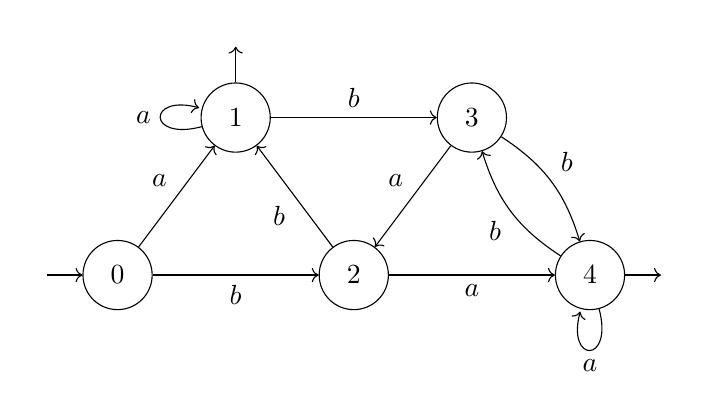
\begin{tikzpicture}[node distance = 3cm, on grid, auto]
      \node[state, initial] (q0)   {$0$};
      \node[state, accepting above] (q1) [above right = 2cm and 1.5cm of q0]  {$1$};
      \node[state] (q2) [below right = 2cm and 1.5cm of q1]  {$2$};
      \node[state] (q3) [above right = 2cm and 1.5cm of q2]  {$3$};
      \node[state, accepting right] (q4) [below right = 2cm and 1.5cm of q3]  {$4$};
      
      \path[->]
        (q0) edge node[below] {$b$} (q2)
          edge node {$a$} (q1)
        (q1) edge[loop left] node {$a$} (q1)
          edge node {$b$} (q3)
        (q2) edge node {$b$} (q1)
          edge node[below] {$a$} (q4)
        (q3) edge node[above left] {$a$} (q2)
          edge[bend left=20] node {$b$} (q4)
        (q4) edge[loop below] node {$a$} (q4)
          edge[bend left=20] node {$b$} (q3);
     \end{tikzpicture}
  \end{center}

\clearpage

\section*{Exercice 2 : Résiduels}

  L'automate minimal du langage $L = (b(aa)^*b)^*$ a 4 états. Déterminez
  tous les résiduels de $L$, en écrivant les langages qu'ils
  représentent, et donnez l’automate des résiduels ainsi obtenu.

\vfill

\section*{Exercice 3 : Non-régularité}

  Montrez que le langage $L=\{ a^{n} b^{2n} \mid n \geq 0\}$ n'est pas régulier. Vous pouvez
  soit utiliser les résiduels, soit le lemme de pompage.


   \noindent Pour rappel, la contraposée du lemme de pompage est :
   \begin{quote}
    Soit $L$ un langage. 
   Si pour tout $N >0$, il existe un mot $x \in L$ de longueur au moins
   $N$ et tel que pour toute décomposition $x=uvw$ avec $v
   \neq\varepsilon$ et $|uv| <N$, il existe un $k \ge 0$ tel que $u\,
   v^k \, w \notin L$, alors $L$ n'est pas régulier.
   \end{quote}

\vfill

\end{document}
